\documentclass{article}
\usepackage[utf8]{inputenc}
\usepackage[T1]{fontenc}
\usepackage[english]{babel}
\setlength{\parindent}{0pt}
\usepackage{hyperref}
\hypersetup{
    colorlinks=true,
    linkcolor=blue,
    filecolor=magenta,      
    urlcolor=cyan}
\usepackage{graphicx}
\graphicspath{ {./pic/} }

\usepackage{fourier,amssymb,microtype,amsmath,gensymb}
\newcommand{\R}{\mathbb{R}}
\usepackage{mdframed,caption,xcolor}
\usepackage{tikz,tkz-euclide}

\title{Seminar 1 - Preference and Marshallian demand function}
\author{Xiaoguang Ling \\  \href{xiaoguang.ling@econ.uio.no}{xiaoguang.ling@econ.uio.no}}
\date{\today}

\begin{document}

\maketitle

%%%%%%%%%%%%%%%%%%%%%%%%%%%%%%%%%%%%%%%%%%%%%%%%%%%%%%%%%%%%%%%%%%%%%%%%%%%%%%%%%%%%%%%%%%%%%%
\section*{Before we start}

\begin{itemize}
\item The course/seminar is difficult and time-consuming $\rightarrow$ help each other
\item More details on assumptions we have used in previous economic classes, more complex and interesting questions, more mathematics 
\item Use your textbook wisely: Hints, Mathematical Appendices, Index
\item Open-book exam, can also be difficult. Previous exam: \href{https://www.uio.no/studier/emner/sv/oekonomi/ECON4220/previous-exams/}{Econ 4220/3220}, \href{https://www.uio.no/studier/emner/sv/oekonomi/ECON3200/previous-exams/index.html}{Econ 4200/3200}
\item Zoom seminars, solution sketch will be available before every weekend in Canvas.
\item Your feedback is important (too fast, unclear, mistakes etc.). Contact me (\href{xiaoguang.ling@econ.uio.no}{xiaoguang.ling@econ.uio.no}) in time!
\end{itemize}

\newpage

\section*{One more thing about online teaching}
Your in-time feedback (questions,suggestions,criticism, etc.) really matters, especially at these times.

Here are several ways for online Q \& A 
\begin{itemize}
\item \href{https://www.dropbox.com/referrals/AACx30a_-sudYoShl6zfNAQGKT2agvs-2wY?src=global9}{Dropbox} folder sharing. I'll show you how to ask questions on it .
\begin{itemize}
\item Free, no downloading needed
\item You can comment on my slides directly, and point out in which line/graph/fuction the problem is.
\item Email address needed(to permit you editing my folder), sign your Email address here if you want: \href{https://docs.google.com/spreadsheets/d/1pNukxmwu8BX5blj0uOcLB7XxZX7gxgjpQsle1yO1vZI/edit?usp=sharing}{GoogleSheet}
\end{itemize}

\item Zoom meeting. Maybe we can arrange online office hours.
\item Email. Do contact us before it's too late, don't hesitate
\end{itemize}

\bigskip

As you may know, your questions can contain many graphs and mathematical symbols, here are ways to make them online:

\begin{itemize}
\item Photo of your handwrittings.
\item Record your questions and send it to me
\item Write it in \LaTeX{} format and send me your text (I will appreciate it :) )
\end{itemize}

\bigskip

We will create a new document called "Q\&A.pdf" in our shared folder. It will contain all the questions
We collected from you and my answers.
\begin{itemize}
\item Questions will be anonymous without special requirement.
\end{itemize}

\newpage

\section*{A Road map for this semester}

\bigskip

\bigskip


\usetikzlibrary{arrows,shapes,positioning,shadows,trees}
\tikzset{
  basic/.style  = {draw, text width=2cm, drop shadow, font=\sffamily, rectangle},
  root/.style   = {basic, rounded corners=2pt, thin, align=center,
                   fill=green!30},
  level 2/.style = {basic, rounded corners=6pt, thin,align=center, fill=green!60,
                   text width=8em},
  level 3/.style = {basic, thin, align=left, fill=pink!60, text width=6.5em}
}

\begin{tikzpicture}[
  level 1/.style={sibling distance=40mm},
  edge from parent/.style={->,draw},
  >=latex]

\node[root] {Econ 3220/4220}
  child {node[level 2] (c1) {Economic Agents}}
  child {node[level 2] (c2) {Equilibrium}}
  child {node[level 2] (c3) {Game Theory}}
  child {node[level 2] (c4) {More about Information}};

\begin{scope}[every node/.style={level 3}]
\node [below of = c1, xshift=15pt] (c11) {Consumer};
\node [below of = c11] (c12) {Firm};

\node [below of = c3, xshift=15pt] (c31) {Static};
\node [below of = c31] (c32) {Dynamic};
\node [below of = c32] (c33) {Complete information};
\node [below of = c33] (c34) {Incomplete information};

\node [below of = c4, xshift=15pt] (c41) {Moral Hazard};
\node [below of = c41] (c42) {Adverse Selection};
\node [below of = c42] (c43) {Bidding in Auctions};

\end{scope}

\foreach \value in {1,2}
  \draw[->] (c1.195) |- (c1\value.west);

\foreach \value in {1,2,3,4}
  \draw[->] (c3.195) |- (c3\value.west);

\foreach \value in {1,2,3}
  \draw[->] (c4.195) |- (c4\value.west);


\end{tikzpicture}

\newpage
%%%%%%%%%%%%%%%%%%%%%%%%%%%%%%%%%%%%%%%%%%%%%%%%%%%%%%%%%%%%%%%%%%%%%%%%%%%%%%%%%%%%%%%%%%%%%%

\section{Jehle \& Reny 1.8. Axioms of consumer choice}

Sketch a map of indifference sets that are all \textbf{parallel}, \textbf{negatively sloped 
straight lines}, with \textbf{preference increasing north-easterly}.We know that preferences 
such as these satisfy Axioms 1, 2, 3, and 4. 
\begin{itemize}
\item Prove that they also satisfy Axiom 5'. 
\item Prove that they do not satisfy Axiom 5.
\end{itemize}

\begin{mdframed}[backgroundcolor=blue!20,linecolor=white] 

\textbf{Review: 5 Axioms of consumer choice (JR pp. 5-12)}

\vspace{2mm}

The preference (indifference curve) shown in Figure \ref{fig:familiar} is classical in all
economics classes. Why does it look like this way?

\vspace{2mm}

{\centering
\begin{tikzpicture}[scale=1.2]
\draw [->] (0,0) node [below] {0} -- (0,0) -- (5.5,0) node [below] {$x_1$};
\draw [->] (0,0) node [below] {0} -- (0,0) -- (0,5.5) node [left] {$x_2$};

\draw (0.3,5) to [out=280,in=175] (5.5,0.5);
\draw (1,5) to [out=280,in=175] (5.5,1.2);
\draw (1.6,5) to [out=280,in=175] (5.5,1.8);
\end{tikzpicture}
\captionof{figure}{An indifference map}
\label{fig:familiar}}
\vspace{2mm}

The most basic assumptions about our preference are Axiom 1.  and Axiom 2. 

\begin{itemize}
\item Axiom 1. Completeness (We can always choose)
$\forall \ x^1, x^2$ in $X$, we have: $x^1 \succsim  x^2$ or $x^2 \succsim  x^3$  or both
\item Axiom 2. Transitivity
$\forall \ x^1, x^2$, and  $x^3$ in $X$, if $x^1 \succsim  x^2$ and $x^2 \succsim  x^3$, then $x^1 \succsim  x^3$
\end{itemize}

With Axiom 1. and Axiom 2. , the preference set can be:

\vspace{2mm}

{\centering
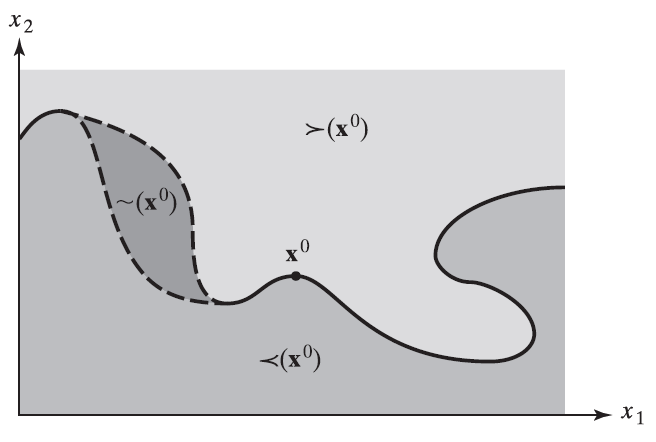
\includegraphics[width=0.8\textwidth]{1.open}
\captionof{figure}{Hypothetical preferences satisfying Axioms 1 and 2.}
\label{open}}
\vspace{2mm}

What happens around the "boundary"?

\begin{itemize}
\item Axiom 3. Continuity (define boundary)

$\succsim (x)$ and $\precsim (x)$ sets are closed in $\R^n_+$ for $x \in \R^n_+ $.
\end{itemize}

Once the boundary is properly defined, there is no sudden preference reversal any more.
Now the preference set looks like Figure \ref{fig:ball}

\vspace{2mm}

{\centering
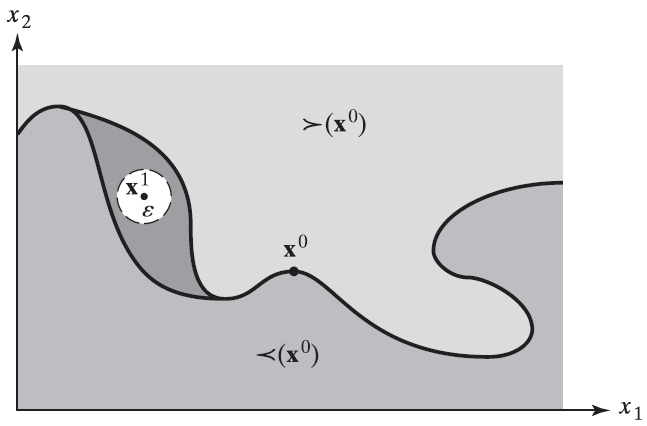
\includegraphics[width=0.8\textwidth]{1.ball}
\captionof{figure}{Hypothetical preferences satisfying Axioms 1, 2, and 3.}
\label{fig:ball}}

\vspace{2mm}

Further more, we assume "unlimited wants" can be represented by our preference.
For example, we can try Axiom 4'.

\begin{itemize}
\item Axiom 4'. Local non-satiation (always something better around)

$\forall \ x^0 \in \R^n_+ \ $ and $ \ \forall \ \epsilon > 0$, $\exists x 
\in B_{\epsilon}(x^0) \cap \R^n_+ \ $ s.t. $\ x \succ x^0$
\end{itemize}


Axiom 4' rulled out the "indifference zone" in Figure \ref{fig:ball} and our preference set
is deduced into Figure \ref{fig:line}.
\vspace{2mm}

{\centering
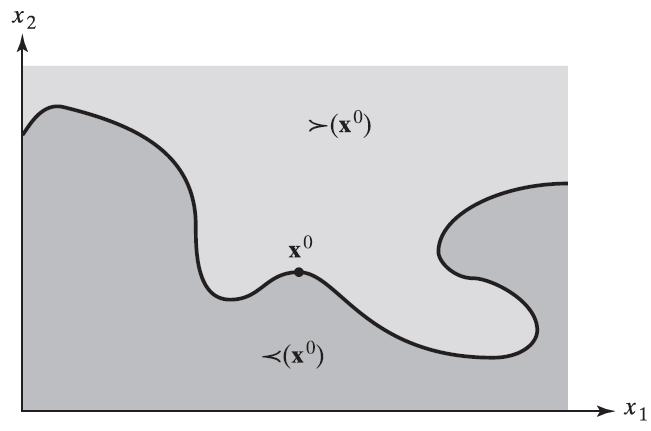
\includegraphics[width=0.8\textwidth]{1.line}
\captionof{figure}{Hypothetical preferences satisfying Axioms 1, 2, 3 and 4'}
\label{fig:line}}
\vspace{2mm}

However, Axiom 4' doesn't mean "the more, the better (at least not worse)" shown in Figure \ref{fig:mono}.
\vspace{2mm}

{\centering
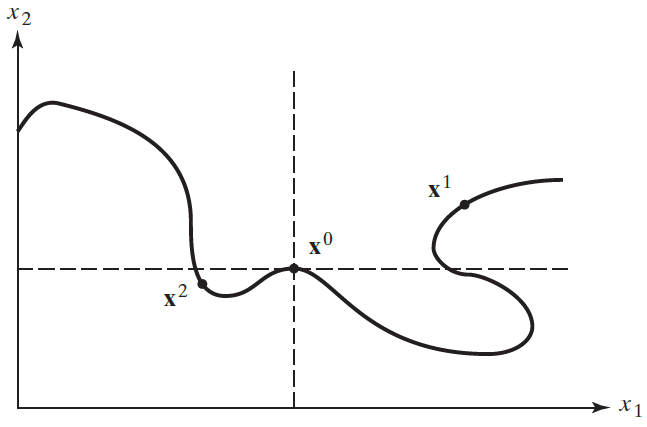
\includegraphics[width=0.8\textwidth]{1.mono}
\captionof{figure}{Hypothetical preferences satisfying Axioms 1, 2, 3 and 4' again}
\label{fig:mono}}
\vspace{2mm}

To depict this, we assume Axiom 4 instead.

\begin{itemize}
\item Axiom 4. Strict monotonicity (the more, the better)

$\forall \ x^0, x^1 \in \R^n_+ \ $, if $x^0 \ge x^1, \ $ then  $\ x^0 \succsim x^1 \ $, while if 
$x^0 \gg x^1, \ $ then  $\ x^0 \succ x^1$.
\end{itemize}

A set of preferences satisfying Axioms 1, 2, 3, and 4 is given in Figure \ref{fig:closest}
\vspace{2mm}

{\centering
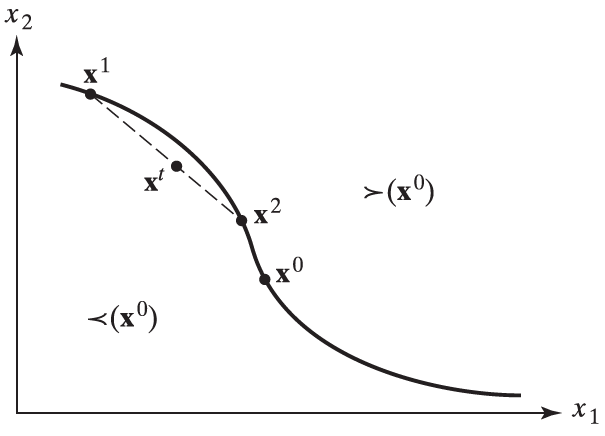
\includegraphics[width=0.8\textwidth]{1.closest}
\captionof{figure}{Hypothetical preferences satisfying Axioms 1, 2, 3 and 4}
\label{fig:closest}}
\vspace{2mm}

In addition, we assume people prefer "balanced" than "extreme" bundles in consumption.
Either Axiom 5' or Axiom 5 can guarantee this, but Axiom 5 will make our analysis easier in the future.

\begin{itemize}

\item Axiom 5'. Convexity

If $\ x^1 \succsim x^0 \ $, then $\ tx^1 + (1-t)x^0 \succsim x^0 \ $ for all $\ t \in [0,1]$

\item Axiom 5. Strict convexity

If $\ x^1 \ne x^0 \ $ and $\ x^1 \succsim x^0 \ $, then $\ tx^1 + (1-t)x^0 \succ x^0 \ $ for all $\ t \in (0,1)$

\end{itemize}

Both Axiom 5' and Axiom 5 can rule out the concave-to-the-origin segments in Figure \ref{fig:closest}.
Finally, we our indifference curve looks the same as in Figure \ref{fig:familiar} and Figure \ref{fig:final}

\vspace{2mm}

{\centering
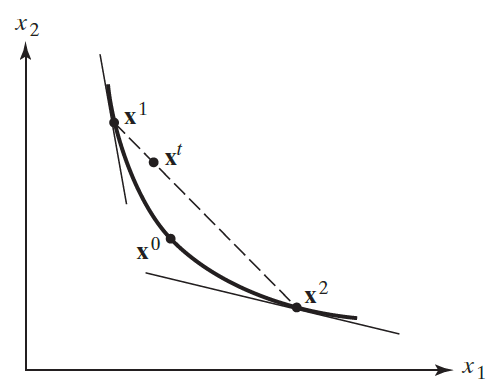
\includegraphics[width=0.8\textwidth]{1.final}
\captionof{figure}{Hypothetical preferences satisfying Axioms 1, 2, 3, 4 and 5'/5}
\label{fig:final}}

\end{mdframed}

As required by question 1.8, a map of the indifference sets is showed in Figure \ref{fig:1_8}

{\centering
\begin{tikzpicture}[scale=0.85]
\draw [->] (0,0) node [below] {0} -- (0,0) -- (9,0) node [below] {$x_1$};
\draw [->] (0,0) node [below] {0} -- (0,0) -- (0,6) node [left] {$x_2$};

\draw [thick] (1,1.5) -- (3,0.5);
\draw [thick] (1,2.5) -- (5,0.5);
\draw [thick] (1,3.5) -- (7,0.5);
\draw [thick] (1,5.5) -- (8,2);

\end{tikzpicture}
\captionof{figure}{A map of the indifference sets for Q.1.8}
\label{fig:1_8}}

%***************************************************
\subsection{Prove that they also satisfy Axiom 5'}

\begin{mdframed}[backgroundcolor=blue!20,linecolor=white] 
Read JR. pp. 501 for the definition Convex combination.
\end{mdframed}

For any given bundle $x^0$ in Figure \ref{fig:1_8_a5'}, we can always
find another bundle $x^1$ either on the same indifference curve with $x^0$ lying on
or to the northeast of $x^0$ s.t. $x^1 \succsim x^0$.

No matter which case, the convex combination of $x^0$ and $x^1$ is always at least 
as good as $x^0$


{\centering
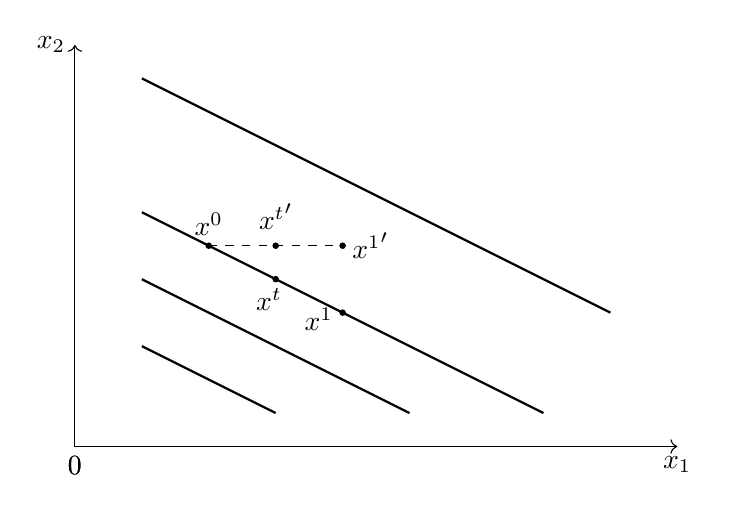
\begin{tikzpicture}[scale=0.85]
\draw [->] (0,0) node [below] {0} -- (0,0) -- (9,0) node [below] {$x_1$};
\draw [->] (0,0) node [below] {0} -- (0,0) -- (0,6) node [left] {$x_2$};


\draw [thick] (1,1.5) -- (3,0.5);
\draw [thick] (1,2.5) -- (5,0.5);
\draw [thick] (1,3.5) -- (7,0.5);
\draw [thick] (1,5.5) -- (8,2);

\node[above] at (2,3) {$x^0$};
\draw[fill] (2,3) circle [radius =0.04];

\node[left] at (4,1.9) {$x^1$};
\draw[fill] (4,2) circle [radius =0.04];

\node[right] at (4,3) {${x^1}'$};
\draw[fill] (4,3) circle [radius =0.04];

\draw[dashed](2,3)--(4,2);
\draw[dashed](2,3)--(4,3);

\node[below] at (2.9,2.5) {$x^t$};
\draw[fill] (3,2.5) circle [radius =0.04];

\node[above] at (3,3.1) {${x^t}'$};
\draw[fill] (3,3) circle [radius =0.04];

\end{tikzpicture}
\captionof{figure}{Axiom 5' Convexity}
\label{fig:1_8_a5'}}

%***************************************************
\subsection{Prove that they do not satisfy Axiom 5}

To prove the preferences do not satisfy Axiom 5, we only need to 
give one example of the violation.

In Figure \ref{fig:1_8_a5}, $x^1 \ne x^0$ and $x^1 \succsim x^0$, but
$x^t=tx^1+(1-t)x^0 \nsucc x^0$ for any $t \in (0,1)$

{\centering
\begin{tikzpicture}[scale=0.85]
\draw [->] (0,0) node [below] {0} -- (0,0) -- (9,0) node [below] {$x_1$};
\draw [->] (0,0) node [below] {0} -- (0,0) -- (0,6) node [left] {$x_2$};

\draw [thick] (1,1.5) -- (3,0.5);
\draw [thick] (1,2.5) -- (5,0.5);
\draw [thick] (1,3.5) -- (7,0.5);
\draw [thick] (1,5.5) -- (8,2);

\node[above] at (2,3) {$x^0$};
\draw[fill] (2,3) circle [radius =0.04];
\node[left] at (4,1.9) {$x^1$};
\draw[fill] (4,2) circle [radius =0.04];
\node[below] at (2.9,2.5) {$x^t$};
\draw[fill] (3,2.5) circle [radius =0.04];

\end{tikzpicture}
\captionof{figure}{Violation of Axiom 5 Strict Convexity}
\label{fig:1_8_a5}}

%%%%%%%%%%%%%%%%%%%%%%%%%%%%%%%%%%%%%%%%%%%%%%%%%%%%%%%%%%%%%%%%%%%%%%%%%%%%%%%%%%%%%%%%%%%%%%
\newpage
\section{Jehle \& Reny 1.9 - Leontief preferences}

Sketch a map of indifference sets that are \textbf{all parallel right angles that ‘kink’ on the line $x_1 = x_2$}. If
\textbf{preference increases north-easterly}, these preferences will satisfy Axioms 1, 2, 3, and 4'. 

\begin{itemize}
\item Prove that they also satisfy Axiom 5'. 

\item Do they satisfy Axiom 4? 

\item Do they satisfy Axiom 5?
\end{itemize}


{\centering
\begin{tikzpicture}[scale=0.85]
\draw [->] (0,0) node [below] {0} -- (0,0) -- (9,0) node [below] {$x_1$};
\draw [->] (0,0) node [below] {0} -- (0,0) -- (0,6) node [left] {$x_2$};

\draw [thick] (1,6) -- (1,1);
\draw [thick] (1,1) -- (8,1);
\draw [thick] (2,6) -- (2,2);
\draw [thick] (2,2) -- (8,2);
\draw [thick] (4,6) -- (4,4);
\draw [thick] (4,4) -- (8,4);

\draw[dashed](0,0)--(5,5);
\node[right] at (5,5) {$x^1=x^2$};

\end{tikzpicture}
\captionof{figure}{A map of the indifference sets for Q.1.9}
\label{fig:1_9}}

%***************************************************
\subsection{Prove that they also satisfy Axiom 5'}

{\centering
\begin{tikzpicture}[scale=0.85]
\draw [->] (0,0) node [below] {0} -- (0,0) -- (9,0) node [below] {$x_1$};
\draw [->] (0,0) node [below] {0} -- (0,0) -- (0,6) node [left] {$x_2$};

\draw [thick] (1,6) -- (1,1);
\draw [thick] (1,1) -- (8,1);
\draw [thick] (2,6) -- (2,2);
\draw [thick] (2,2) -- (8,2);
\draw [thick] (4,6) -- (4,4);
\draw [thick] (4,4) -- (8,4);

\node[right] at (2,5) {$x^0$};
\draw[fill] (2,5) circle [radius =0.04];

\node[right] at (2,3) {$x^1$};
\draw[fill] (2,3) circle [radius =0.04];

\node[right] at (3.5,3) {${x^1}'$};
\draw[fill] (3.5,3) circle [radius =0.04];

\draw[dashed](2,5)--(2,3);
\draw[dashed](2,5)--(3.5,3);

\node[left] at (2,4) {$x^t$};
\draw[fill] (2,4) circle [radius =0.04];

\node[right] at (3,3.7) {${x^t}'$};
\draw[fill] (3,3.67) circle [radius =0.04];

\end{tikzpicture}
\captionof{figure}{Axiom 5' Convexity }
\label{fig:1_9_a5'}}

%***************************************************
\subsection{Do they satisfy Axiom 4?}

Yes. Any bundle ${x^0}'$ that contains at least as much of every good as $x^1$ does
(i.e. ${x^0}' \ge x^1$ )can only lies in the shaded area including the border. 
Obviously, ${x^0}' \succsim x^1$.

In addition, for any ${x^0}$ contains strictly more of every good than $x^1$ 
does (i.e. ${x^0}' \gg x^1$ ), we have ${x^0} \succ x^1$

{\centering
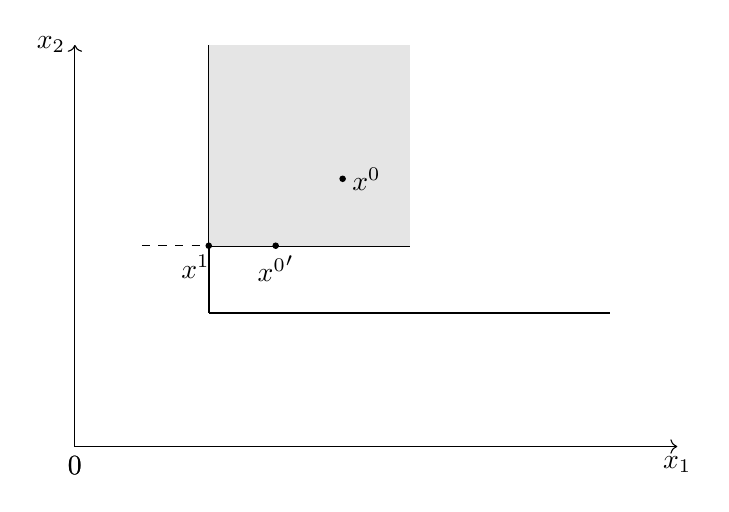
\begin{tikzpicture}[scale=0.85]
\draw [->] (0,0) node [below] {0} -- (0,0) -- (9,0) node [below] {$x_1$};
\draw [->] (0,0) node [below] {0} -- (0,0) -- (0,6) node [left] {$x_2$};

\draw [thick] (2,6) -- (2,2);
\draw [thick] (2,2) -- (8,2);
\draw [thick] (2,3) -- (5,3);
\draw [dashed] (1,3) -- (2,3);
\fill [gray!20] (2.01,3) rectangle (5,6);
\node[below] at (1.8,3) {$x^1$};
\draw[fill] (2,3) circle [radius =0.04];
\node[right] at (4,4) {$x^0$};
\draw[fill] (4,4) circle [radius =0.04];
\node[below] at (3,3) {${x^0}'$};
\draw[fill] (3,3) circle [radius =0.04];


\end{tikzpicture}
\captionof{figure}{Axiom 4 Strict Monotonicity}
\label{fig:1_9_a4}}

%***************************************************
\subsection{Do they satisfy Axiom 5?}

No. In Figure \ref{fig:1_9_a5}, $x^1 \ne x^0$ and $x^1 \succsim x^0$, but
$x^t=tx^1+(1-t)x^0 \nsucc x^0$ for any $t \in (0,1)$


{\centering
\begin{tikzpicture}[scale=0.85]
\draw [->] (0,0) node [below] {0} -- (0,0) -- (9,0) node [below] {$x_1$};
\draw [->] (0,0) node [below] {0} -- (0,0) -- (0,6) node [left] {$x_2$};
\draw [thick] (2,5.6) -- (2,2);
\draw [thick] (2,2) -- (8,2);
\node[left] at (1.8,3) {$x^1$};
\draw[fill] (2,3) circle [radius =0.04];
\node[left] at (2,5) {$x^0$};
\draw[fill] (2,5) circle [radius =0.04];
\node[right] at (2,4) {${x^t}$};
\draw[fill] (2,4) circle [radius =0.04];
\end{tikzpicture}
\captionof{figure}{Axiom 5 Strict Convexity}
\label{fig:1_9_a5}}


%%%%%%%%%%%%%%%%%%%%%%%%%%%%%%%%%%%%%%%%%%%%%%%%%%%%%%%%%%%%%%%%%%%%%%%%%%%%%%%%%%%%%%%%%%%%%%
\section{Jehle \& Reny 1.13 - Lexicographic preferences}
A consumer has lexicographic preferences over $\R^2_+$ if the relation  satisfies $x_1, x_2$ whenever
$x_1^1 > x_1^2$, or $x_1^1 = x_1^2$ and $x_1^1 \ge x_1^2$.

\begin{itemize}
\item Sketch an indifference map for these preferences.
\item Can these preferences be represented by a continuous utility function? Why or why not?
\end{itemize}

\begin{mdframed}[backgroundcolor=blue!20,linecolor=white]
$\forall x^1,x^2 \in \R^2_+$, Lexicographic preferences can be defined as:
\begin{equation}
x^1 \succsim x^2 \Leftrightarrow
    \begin{cases}
      \text{$x^1_1 > x^2_1$}\\
      \text{or}\\
      \text{$x^1_1 = x^2_1 \ and \ x^1_2 \ge x^2_2$}\\
    \end{cases}
    \label{eq:laxi}  
\end{equation}
\begin{itemize}
\item $x_1$ is critical
\item like a dictionary
\end{itemize}
\end{mdframed}

%***************************************************
\subsection{Sketch an indifference map for these preferences.}
There is no indifference map for Lexicographic preferences. To draw the indifference map,
we must have different bundles lying on indifference curves.

Assume there are two different budles $x^1, x^2$ s.t. $x^1 \sim x^2$, i.e. $x^1 \succsim x^2$
and $x^2 \succsim x^1$. According to the definition in formula \ref{eq:laxi}, this requires
\begin{equation}
    Both \
    \begin{cases}
      \text{$x^1_1 > x^2_1$}\\
      \text{or}\\
      \text{$x^1_1 = x^2_1 \ and \ x^1_2 \ge x^2_2$}\\
    \end{cases}
    and \ 
    \begin{cases}
      \text{$x^2_1 > x^1_1$}\\
      \text{or}\\
      \text{$x^2_1 = x^1_1 \ and \ x^2_2 \ge x^1_2$}\\
    \end{cases}
    \label{eq:nomap}   
\end{equation}

Obviously, the only possible condition is $x^1_1 = x^2_1 \ and \ x^1_2 = x^2_2$, which contradicts
with our assertion $x^1, x^2$ are different.

%***************************************************
\subsection{Can these preferences be represented by a continuous utility function? Why or why not?}

No. Because Lexicographic preferences are not continuous. 

According to our Axiom 3, continuity means $\succsim$ and $\precsim$ sets are closed. 
In Figure \ref{fig:1_13_pre}, we can see the $\succsim$ set for any bundle $x^0$ is not closed.

{\centering
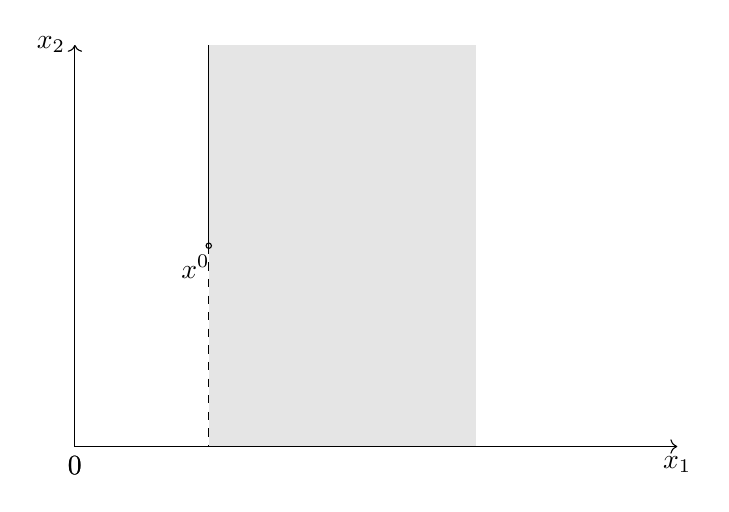
\begin{tikzpicture}[scale=0.85]
\draw [->] (0,0) node [below] {0} -- (0,0) -- (9,0) node [below] {$x_1$};
\draw [->] (0,0) node [below] {0} -- (0,0) -- (0,6) node [left] {$x_2$};

\draw [thick] (2,3) -- (2,6);
\draw [dashed] (2,3) -- (2,0);
\fill [gray!20] (2.01,0.01) rectangle (6,6);
\node[below] at (1.8,3) {$x^0$};
\draw (2,3) circle [radius =0.04];

\end{tikzpicture}
\captionof{figure}{${\succsim x^0}$ set for Lexicographic preferences}
\label{fig:1_13_pre}}

\vspace{2mm}

%%%%%%%%%%%%%%%%%%%%%%%%%%%%%%%%%%%%%%%%%%%%%%%%%%%%%%%%%%%%%%%%%%%%%%%%%%%%%%%%%%%%%%%%%%%%%%
\section{Jehle \& Reny 1.15 - compact and convex}
Prove that the budget set, $B$, is a \textbf{compact, convex set whenever $p \gg 0$}.

\begin{mdframed}[backgroundcolor=blue!20,linecolor=white]
\begin{itemize}
\item A budget set $B$ can be difined as $B \equiv {x \in \R^n_+ | p_1x_1 + p_2x_2 + \ldots + p_nx_n \le y}$
\item \begin{equation}
 S \  \ is \ \ Compact \ (JR. \ pp. 514):
    \begin{cases}
      \text{Closed: not open}\\
      \text{Bounded: $\exists \epsilon > 0 \ $ s.t. $\ S \subset B_{\epsilon}(x)$}\\
    \end{cases}
    \end{equation}

\item Open:  $S$ is open if $\forall x \in S, \exists \epsilon > 0 \ $ s.t. $\ B_{\epsilon}(x) \subset S$ \\
\item Convex: $S$ is convex if for any $x^1, x^2 \in S,\ $ we have $tx^1 + (1-t)x^2 \in S, \forall t \in [0,1]$
\end{itemize}
\end{mdframed}

%***************************************************
\subsection{Budget set $B$ is compact when $p \gg 0$}

\textbf{(1) $B$ is closed(not open).}


{\centering
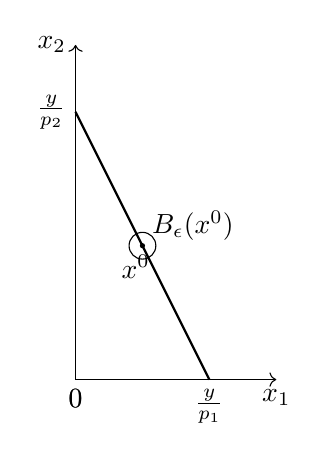
\begin{tikzpicture}[scale=0.85]
\draw [->] (0,0) node [below] {0} -- (0,0) -- (3,0) node [below] {$x_1$};
\draw [->] (0,0) node [below] {0} -- (0,0) -- (0,5) node [left] {$x_2$};
\draw [thick] (0,4) -- (2,0);
\draw (1,2) circle [radius =0.2];
\draw [fill] (1,2) circle [radius =0.03];
\node[right] at (1,2.3) {$B_{\epsilon}(x^0)$};
\node[below] at (0.9,2) {$x^0$};
\node[below] at (2,0) {$\frac{y}{p_1}$};
\node[left] at (0,4) {$\frac{y}{p_2}$};

\end{tikzpicture}
\captionof{figure}{An example of closed budget set with 2 dimentions}
\label{fig:1_15_close}}

\vspace{2mm}

We can find some $x^0$, s.t. $p'x^0 = p_1x^0_1 + p_2x^0_2 + \ldots + p_nx^0_n = y$.

Where $p' = (p_1, p_2, \ldots, p_n)$ and ${x^0}' = (x^0_1, x^0_2, \ldots, x^0_n)$

Obviously, $x^0 \in  S$ (actually it's on the boundary).

\medskip

Define $B_{\epsilon}(x^0)$ as the ball with $x^0$ as center and $\epsilon > 0$ as radius.

For any $\epsilon > 0 \ $, we can always find some $ \ e \in (0, \epsilon) \ $ s.t. bundle 
$\ x^1 = (x^0_1 + e, x^0_2, \ldots, x^0_n)$ lies in ball $B_{\epsilon}(x^0)$, while since $\ p'x^1 > y$, 
$x^1$ is out of the budget set $B$.

\medskip

In conclusion: we can never find an $\epsilon > 0 \ $ s.t. $\ B_{\epsilon}(x^0) \subset B$. Therefore
$B$ is closed.

\bigskip

\textbf{(2) $B$ is bounded}

Define $N \equiv max\{\frac{y}{p_1},\frac{y}{p_2},\ldots, \frac{y}{p_n}\} > 0$.

$\forall x \in B$, we have $C = (N,N, \ldots, N) > x$. We can thus argue that $B$
can be contained by some ball  $B_{(\epsilon)}(x^0)$, i.e. bounded.

\begin{mdframed}[backgroundcolor=blue!20,linecolor=white]
For example:

{\centering
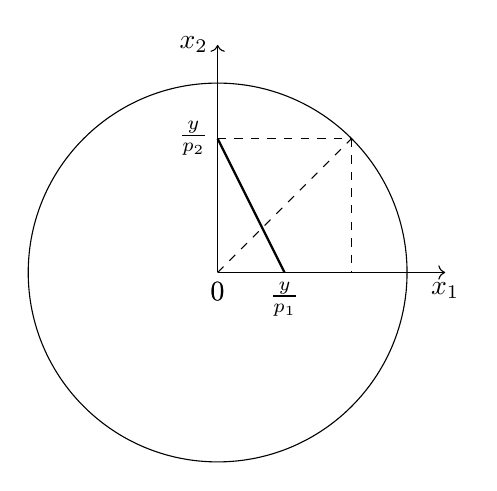
\begin{tikzpicture}[scale=0.85]
\draw [->] (0,0) node [below] {0} -- (0,0) -- (3.4,0) node [below] {$x_1$};
\draw [->] (0,0) node [below] {0} -- (0,0) -- (0,3.4) node [left] {$x_2$};
\draw [thick] (0,2) -- (1,0);
\draw [dashed] (2,2) -- (2,0);
\draw [dashed] (0,2) -- (2,2);
\draw [dashed] (0,0) -- (2,2);
\node[below] at (1,0) {$\frac{y}{p_1}$};
\node[left] at (0,2) {$\frac{y}{p_2}$};
\draw (0,0) circle [radius =2.83];
\end{tikzpicture}
\captionof{figure}{An example of closed budget set with 2 dimentions}
\label{fig:1_15_bounded}}

\vspace{2mm}

$B \subset C \subset B_{(nN^n)^{\frac{1}{n}}}(origin)$.
\end{mdframed}

%***************************************************
\subsection{Budget set $B$ is convex when $p \gg 0$}

Again, define price vector $p' = (p_1, p_2, \ldots, p_n)$ and bundle ${x}' = (x_1, x_2, \ldots, x_n)$

For any $x^1, x^2 \in B$, we have 
\begin{align*}  
     p'x^1 \le y \\
     p'x^2 \le y \\
\end{align*}

Define $x^t = tx^1 + (1-t)x^2, t \in [0,1]$

We have 
\begin{align*}  
  p'x^t &=  p'tx^1 +  p'(1-t)x^2 \\
        &=  tp'x^1 +  (1-t)p'x^2 \\
        &\le  ty +  (1-t)y \\
\end{align*}

$p'x^t \le y \Rightarrow x^t \in B$. Therefore $B$ is compact.

%%%%%%%%%%%%%%%%%%%%%%%%%%%%%%%%%%%%%%%%%%%%%%%%%%%%%%%%%%%%%%%%%%%%%%%%%%%%%%%%%%%%%%%%%%%%%%
\section{Jehle \& Reny 1.26 - Marshallian demand function}
A consumer of \textbf{two goods} faces \textbf{positive prices} and has a \textbf{positive income}. 
His utility function is $$u(x_1, x_2) = x_1$$ 
\begin{itemize}
\item Derive the Marshallian demand functions.
\end{itemize}

\begin{mdframed}[backgroundcolor=blue!20,linecolor=white]
Marshallian demand functions $x^* = x(p, y)$ is the solutions 
to the utility maximisation problem (JR. pp.21).
\end{mdframed}

Here we have a 2-commodities consumption problem:

\begin{equation}
  \begin{cases}
  Commodities: x_1, x_2 \ge 0 \\
  Price: p_1, p_2 > 0 \\
  Income: y > 0 \\
  Utility: u(x_1,x_2) = x_1 \\
  
  \end{cases}
\end{equation}

A consumer wants to 
$$\max_{x_1,x_2} \ u(x_1,x_2) = x_1 \ \ s.t. \ p_1x_1 + p_2x_2 \le y,
\ \ and \ x_1, x_2 \ge 0 $$

{\centering
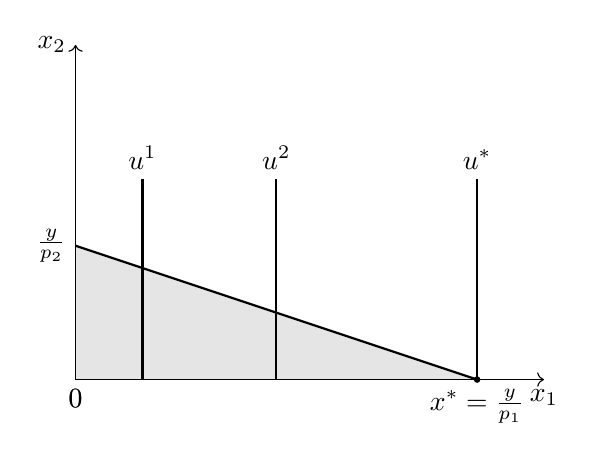
\begin{tikzpicture}[scale=0.85]
\draw [->] (0,0) node [below] {0} -- (0,0) -- (7,0) node [below] {$x_1$};
\draw [->] (0,0) node [below] {0} -- (0,0) -- (0,5) node [left] {$x_2$};
\draw [fill=gray!20] (0,2) -- (0,0) -- (6,0);

\draw [thick] (0,2) -- (6,0);
\draw [thick] (1,3) -- (1,0);
\draw [thick] (3,3) -- (3,0);
\draw [thick] (6,3) -- (6,0);

\node[above] at (1,3) {$u^1$};
\node[above] at (3,3) {$u^2$};
\node[above] at (6,3) {$u^*$};

\node[below] at (6,0) {$x^* =\frac{y}{p_1}$};
\node[left] at (0,2) {$\frac{y}{p_2}$};
\draw [fill] (6,0) circle [radius =0.04];

\end{tikzpicture}
\captionof{figure}{Corner solution}
\label{fig:1_15_corner}}

\vspace{2mm}

$x_1^*(p_1,y)=\frac{y}{p_1}, x_2^*=0$, note it's a corner solution.


\begin{mdframed}[backgroundcolor=blue!20,linecolor=white]
If you want to use Lagrangian method, be sure don't forget $x_1, x_2 \ge 0$.
This is important for corner solutions.

More general, we can use \href{https://mjo.osborne.economics.utoronto.ca/index.php/tutorial/index/1/ktc/t}{Kuhn-Tucker conditions} to solve the problem.

$\max_{x_1,x_2} \ u(x_1,x_2) =  \ \ s.t. \ p_1x_1 + p_2x_2 \le y,
\ \ and \ x_1, x_2 \ge 0 $ are:
Lagrangian function:
$$L = x_1 + \lambda_1(y - p_1x_1 - p_2x_2) + \lambda_2(x_1-0)+ \lambda_3(x_2-0)$$

The Kuhn-Tucker conditions are:

\begin{equation}
  \begin{cases}
    \frac{\partial L}{\partial x_1} = 1-p_1\lambda_1 + \lambda_2 =0 \\
    \frac{\partial L}{\partial x_1} = -p_2\lambda_1 + \lambda_3 =0 \\
  \end{cases}
  \label{eq:L1}
\end{equation}

\begin{equation}
  \begin{cases}
    p_1x_1 + p_2x_2 \le y \\
    \lambda_1 \ge 0 \\
    \lambda_1(y - p_1x_1 - p_2x_2) =0 \\
  \end{cases}
   \label{eq:L2}
\end{equation}

\begin{equation}
  \begin{cases}
    x_1 \ge y \\
    \lambda_2 \ge 0 \\
    \lambda_2 x_1 =0 \\
  \end{cases}
   \label{eq:L3}
\end{equation}

\begin{equation}
  \begin{cases}
    x_2 \ge y \\
    \lambda_3 \ge 0 \\
    \lambda_3 x_2 =0 \\
  \end{cases}
   \label{eq:L4}
\end{equation}

\begin{itemize}
\item If $x_1,x_2>0$, by condition \ref{eq:L3} and \ref{eq:L4}, $\lambda_2 = \lambda_3 =0$.
Contradicts with condition \ref{eq:L1}

\item If $x_1=0,x_2>0$, by condition \ref{eq:L4}, $\lambda_3 =0$.
With condition \ref{eq:L1}, we have $\lambda_1 =0, \lambda_2 = -1$, condition \ref{eq:L3} violated.

\item If $x_1>0,x_2=0$, by condition \ref{eq:L3}, $\lambda_2 =0$.
With condition \ref{eq:L1}, we have $\lambda_1 =\frac{1}{p_1}, \lambda_3 = \frac{p_2}{p_1}$.
With condition \ref{eq:L2}, $x_1^* = \frac{y}{p_1}$
\end{itemize}
\end{mdframed}

\begin{mdframed}[backgroundcolor=yellow!20,linecolor=white]
Tips for exam:
\begin{itemize}

\item Drawing a sketch of the budget set and the indifference curves can be very helpful when the utility 
function is "bizarre". See also the next question.

\end{itemize}

\end{mdframed}

%%%%%%%%%%%%%%%%%%%%%%%%%%%%%%%%%%%%%%%%%%%%%%%%%%%%%%%%%%%%%%%%%%%%%%%%%%%%%%%%%%%%%%%%%%%%%%
\section{Jehle \& Reny 1.27 - Masshallian demand function}

A consumer of \textbf{two goods} faces \textbf{positive} prices and has a \textbf{positive income}. 
His utility function is $$u(x_1, x_2) = max[ax_1, ax_2] + min[x_1, x_2], \ \ where \ \ 0 < a < 1.$$
\begin{itemize}
\item Derive the Marshallian demand functions.
\end{itemize}

The utility $u(x_1, x_2) = max[ax_1, ax_2] + min[x_1, x_2]$ depends on the relation between $ax_1, ax_2$ and $x_1, x_2$

Since $0 < a < 1$, we know $ax_1 \ge ax_2 \iff x_1 \ge x_2$. Thus:
\begin{equation}
  \begin{cases}
If \ \ x_2 >= x_1 ,\ \ u(x_1, x_2) = ax_2 + x_1  \\
If \ \ x_1 >= x_2 ,\ \ u(x_1, x_2) = ax_1 + x_2
  \end{cases}
 \label{eq:mm}
\end{equation}

\begin{mdframed}[backgroundcolor=blue!20,linecolor=white]

Any indifference curve in a rectangular coordinate system below is actually the graph of
a function $x_2 = f_(x_1)$

{\centering
\begin{tikzpicture}[scale=0.85]
\draw [->] (0,0) node [below] {0} -- (0,0) -- (2,0) node [below] {$x_1$};
\draw [->] (0,0) node [below] {0} -- (0,0) -- (0,2) node [left] {$x_2$};
\end{tikzpicture}
\captionof{figure}{A rectangular coordinate system}
\label{fig:1_27_coor}}

More specifically, since bundles on the same indifference curve can provide the same level of utility,
an indifference curve is the graph of a function $x_2 = f_(x_1)$ given some utility $\bar{u}$

Given  $u = \bar{u}$, We can rewrite equation \ref{eq:mm} as:

\begin{equation}
  \begin{cases}
    If \ \ x_2 >= x_1 ,\ \ x_2 = -\frac{1}{a}x_1 + \frac{1}{a}\bar{u} \\
    If \ \ x_1 >= x_2 ,\ \ x_2 = -ax_1 + \bar{u} \\
  \end{cases}
\end{equation}

Now we can draw the sketch of the indifference curves:

{\centering
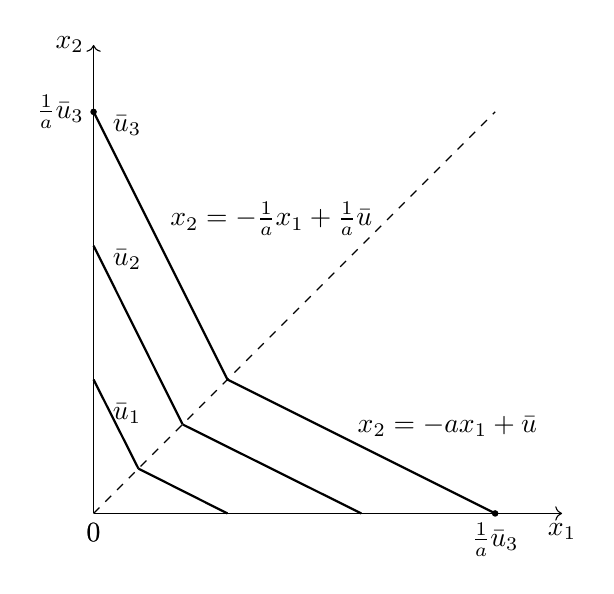
\begin{tikzpicture}[scale=0.85]
\draw [->] (0,0) node [below] {0} -- (0,0) -- (7,0) node [below] {$x_1$};
\draw [->] (0,0) node [below] {0} -- (0,0) -- (0,7) node [left] {$x_2$};

\draw [thick] (0,2) -- (0.67,0.67);
\draw [thick] (0.67,0.67) -- (2,0);
\draw [thick] (0,4) -- (1.33,1.33);
\draw [thick] (1.33,1.33) -- (4,0);
\draw [thick] (0,6) -- (2,2);
\draw [thick] (2,2) -- (6,0);
\draw [dashed] (0,0) -- (6,6);

\node[above] at (0.5,1.2) {$\bar{u}_1$};
\node[above] at (0.5,3.5) {$\bar{u}_2$};
\node[above] at (0.5,5.5) {$\bar{u}_3$};
\node[right] at (1,4.4) {$x_2 = -\frac{1}{a}x_1 + \frac{1}{a}\bar{u}$};
\node[right] at (3.8,1.3) {$x_2 = -ax_1 + \bar{u}$};

\node[below] at (6,0) {$\frac{1}{a}\bar{u}_3$};
\node[left] at (0,6) {$\frac{1}{a}\bar{u}_3$};
\draw [fill] (6,0) circle [radius =0.04];
\draw [fill] (0,6) circle [radius =0.04];

\end{tikzpicture}
\captionof{figure}{Indifference curves are seperated by 45 $\degree \ $line}
\label{fig:1_27_indiff}}

\vspace{2mm}

If we have a budget set similar to the one in Figure \ref{fig:1_27_budget}, we can move our
indifference curve until we have a tangent point. The affordable bundle maximazing the utility
is thus found.

{\centering
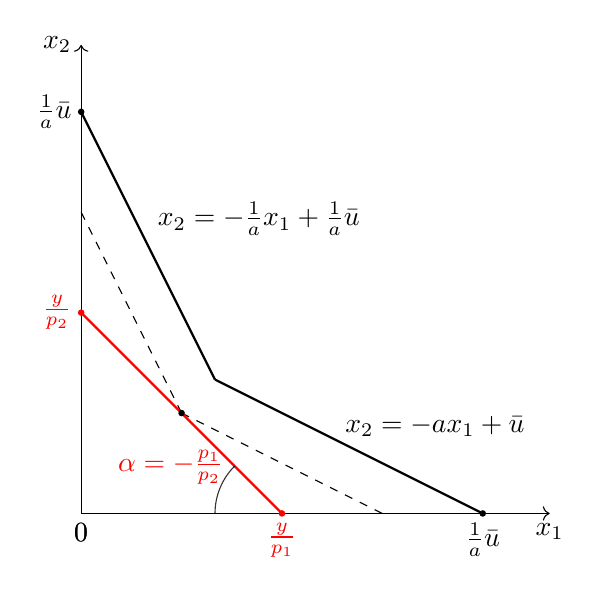
\begin{tikzpicture}[scale=0.85]
\draw [->] (0,0) node [below] {0} -- (0,0) -- (7,0) node [below] {$x_1$};
\draw [->] (0,0) node [below] {0} -- (0,0) -- (0,7) node [left] {$x_2$};

\draw [thick] (0,6) -- (2,2);
\draw [thick] (2,2) -- (6,0);
\draw [dashed] (0,4.5) -- (1.5,1.5);
\draw [dashed] (1.5,1.5) -- (4.5,0);

\draw [thick,red] (0,3) -- (3,0);

\node[right] at (1,4.4) {$x_2 = -\frac{1}{a}x_1 + \frac{1}{a}\bar{u}$};
\node[right] at (3.8,1.3) {$x_2 = -ax_1 + \bar{u}$};

\node[below] at (6,0) {$\frac{1}{a}\bar{u}$};
\node[left] at (0,6) {$\frac{1}{a}\bar{u}$};
\draw [fill] (6,0) circle [radius =0.04];
\draw [fill] (0,6) circle [radius =0.04];

\node[left,red] at (0,3) {$\frac{y}{p_2}$};
\node[below,red] at (3,0) {$\frac{y}{p_1}$};
\draw [fill,red] (3,0) circle [radius =0.04];
\draw [fill,red] (0,3) circle [radius =0.04];
\draw [fill] (1.5,1.5) circle [radius =0.04];

\tkzDefPoint(0,0){A}
\tkzDefPoint(3,0){B}
\tkzDefPoint(0,3){C}
\tkzMarkAngle[fill=yellow,opacity=0.8](C,B,A)
\tkzLabelAngle[pos= 1.8,red](C,B,A){$\alpha = -\frac{p_1}{p_2}$}

\end{tikzpicture}
\captionof{figure}{A budget set example}
\label{fig:1_27_budget}}

However, there can be other tricky conditions, depending on the shape of the budget set.
For example, in Figure \ref{fig:1_27_budget2}

{\centering
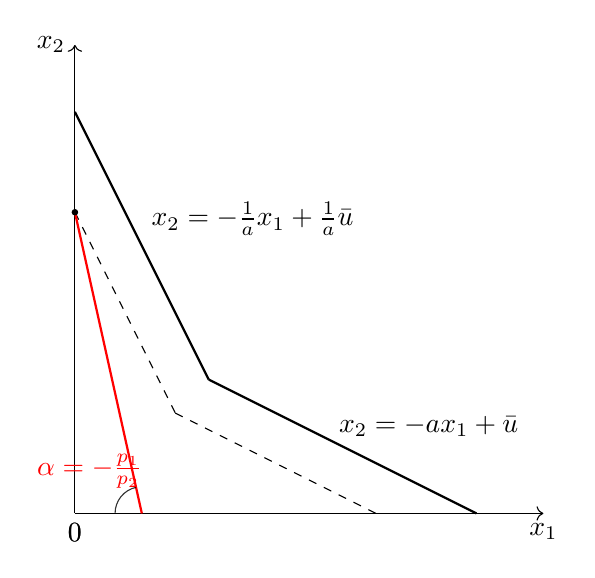
\begin{tikzpicture}[scale=0.85]
\draw [->] (0,0) node [below] {0} -- (0,0) -- (7,0) node [below] {$x_1$};
\draw [->] (0,0) node [below] {0} -- (0,0) -- (0,7) node [left] {$x_2$};

\draw [thick] (0,6) -- (2,2);
\draw [thick] (2,2) -- (6,0);
\draw [dashed] (0,4.5) -- (1.5,1.5);
\draw [dashed] (1.5,1.5) -- (4.5,0);
\node[right] at (1,4.4) {$x_2 = -\frac{1}{a}x_1 + \frac{1}{a}\bar{u}$};
\node[right] at (3.8,1.3) {$x_2 = -ax_1 + \bar{u}$};

\draw [thick,red] (0,4.5) -- (1,0);

\draw [fill] (0,4.5) circle [radius =0.04];

\tkzDefPoint(0,0){A}
\tkzDefPoint(1,0){B}
\tkzDefPoint(0,4.5){C}
\tkzMarkAngle[fill=yellow,size = 0.4, opacity=0.8](C,B,A)
\tkzLabelAngle[pos= 1,red](C,B,A){$\alpha = -\frac{p_1}{p_2}$}

\end{tikzpicture}
\captionof{figure}{A budget set example 2}
\label{fig:1_27_budget2}}
\vspace{2mm}

\begin{itemize}
\item The position of the optimal consumption bundle depends on the slope $\alpha = -\frac{p_1}{p_2}$

\item We need to discussion the relation between $\frac{p_1}{p_2} \ $ and the slop of the 
indifference curve $[a,\frac{1}{a}]$ , for $a \in (0,1)$
\end{itemize}

\end{mdframed}

%***************************************************

\begin{enumerate}

\item When $0 < \frac{p_1}{p_2} < a$, the budget set is showed in Figure \ref{fig:1_27_la}. The Marshallian
demand is $\{x_1 = \frac{y}{p_1}, x_2 = 0\}$

{\centering
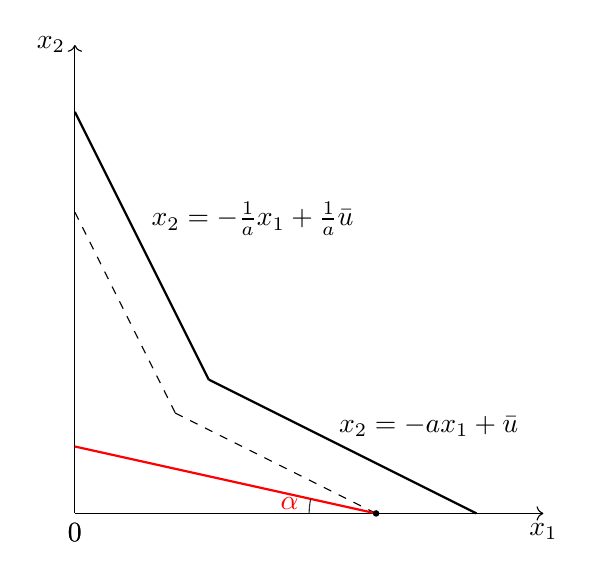
\begin{tikzpicture}[scale=0.85]
\draw [->] (0,0) node [below] {0} -- (0,0) -- (7,0) node [below] {$x_1$};
\draw [->] (0,0) node [below] {0} -- (0,0) -- (0,7) node [left] {$x_2$};

\draw [thick] (0,6) -- (2,2);
\draw [thick] (2,2) -- (6,0);
\draw [dashed] (0,4.5) -- (1.5,1.5);
\draw [dashed] (1.5,1.5) -- (4.5,0);
\node[right] at (1,4.4) {$x_2 = -\frac{1}{a}x_1 + \frac{1}{a}\bar{u}$};
\node[right] at (3.8,1.3) {$x_2 = -ax_1 + \bar{u}$};

\draw [thick,red] (0,1) -- (4.5,0);

\draw [fill] (4.5,0) circle [radius =0.04];

\tkzDefPoint(0,0){A}
\tkzDefPoint(4.5,0){B}
\tkzDefPoint(0,1){C}
\tkzMarkAngle[fill=yellow, opacity=0.8](C,B,A)
\tkzLabelAngle[pos= 1.3,red](C,B,A){$\alpha$}

\end{tikzpicture}
\captionof{figure}{A budget set when $\frac{p_1}{p_2} < a$}
\label{fig:1_27_la}}
\vspace{2mm}


\item When $\frac{p_1}{p_2} = a$, the budget set is showed in Figure \ref{fig:1_27_a}. The Marshallian
demand is in a set $x(p_1,p_2,y) = \{(x_1,x_2)| x_2 \le x_1 and x_2 = -ax_1 + \frac{y}{p_2}\}$


{\centering
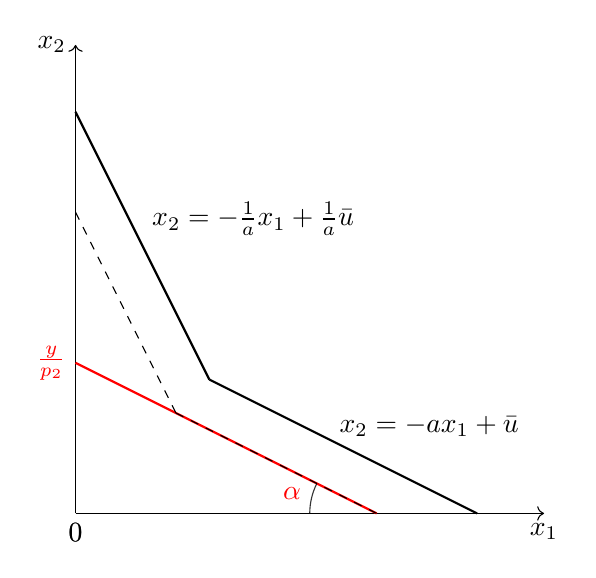
\begin{tikzpicture}[scale=0.85]
\draw [->] (0,0) node [below] {0} -- (0,0) -- (7,0) node [below] {$x_1$};
\draw [->] (0,0) node [below] {0} -- (0,0) -- (0,7) node [left] {$x_2$};

\draw [thick] (0,6) -- (2,2);
\draw [thick] (2,2) -- (6,0);
\node[right] at (1,4.4) {$x_2 = -\frac{1}{a}x_1 + \frac{1}{a}\bar{u}$};
\node[right] at (3.8,1.3) {$x_2 = -ax_1 + \bar{u}$};
\node[left,red] at (0,2.25) {$\frac{y}{p_2}$};

\draw [thick,red] (0,2.25) -- (4.5,0);
\draw [dashed] (0,4.5) -- (1.5,1.5);
\draw [dashed] (1.5,1.5) -- (4.5,0);

\tkzDefPoint(0,0){A}
\tkzDefPoint(4.5,0){B}
\tkzDefPoint(0,2.25){C}
\tkzMarkAngle[fill=yellow, opacity=0.8](C,B,A)
\tkzLabelAngle[pos= 1.3,red](C,B,A){$\alpha$}

\end{tikzpicture}
\captionof{figure}{A budget set when $\frac{p_1}{p_2} = a$}
\label{fig:1_27_a}}
\vspace{2mm}


\item When $\frac{p_1}{p_2} \in (a,\frac{1}{a})$, the budget set was already showed in Figure \ref{fig:1_27_budget}.
In this case, $x_1 = x_2$ and $p_1x_1 + p_2x_2 = y$, the Marshallian demand is therefore
$\{x_1 = \frac{y}{p_1 + p_2}, x_2 = \frac{y}{p_1 + p_2} \}$

{\centering
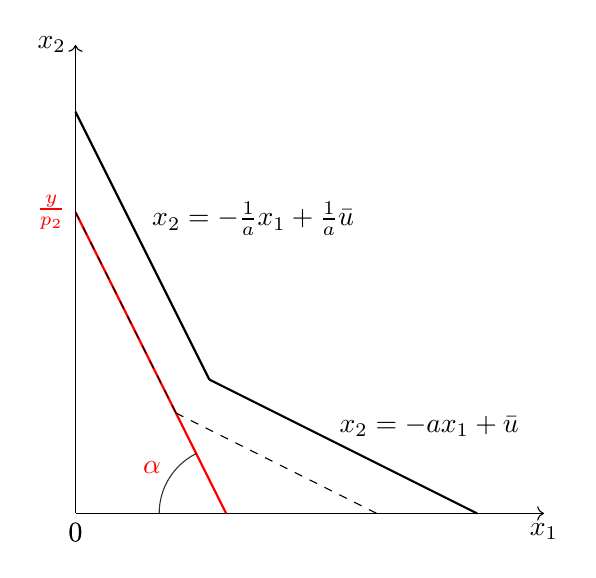
\begin{tikzpicture}[scale=0.85]
\draw [->] (0,0) node [below] {0} -- (0,0) -- (7,0) node [below] {$x_1$};
\draw [->] (0,0) node [below] {0} -- (0,0) -- (0,7) node [left] {$x_2$};

\draw [thick] (0,6) -- (2,2);
\draw [thick] (2,2) -- (6,0);
\node[right] at (1,4.4) {$x_2 = -\frac{1}{a}x_1 + \frac{1}{a}\bar{u}$};
\node[right] at (3.8,1.3) {$x_2 = -ax_1 + \bar{u}$};
\node[left,red] at (0,4.5) {$\frac{y}{p_2}$};

\draw [thick,red] (0,4.5) -- (2.25,0);
\draw [dashed] (0,4.5) -- (1.5,1.5);
\draw [dashed] (1.5,1.5) -- (4.5,0);

\tkzDefPoint(0,0){A}
\tkzDefPoint(2.25,0){B}
\tkzDefPoint(0,4.5){C}
\tkzMarkAngle[fill=yellow, opacity=0.8](C,B,A)
\tkzLabelAngle[pos= 1.3,red](C,B,A){$\alpha$}

\end{tikzpicture}
\captionof{figure}{A budget set when $\frac{p_1}{p_2} = \frac{1}{a}$}\label{fig:1_27_1/a}}
\vspace{2mm}

\item When $\frac{p_1}{p_2} = \frac{1}{a}$, the budget set is showed in Figure \ref{fig:1_27_1/a}. The Marshallian
demand is in a set $x(p_1,p_2,y) = \{(x_1,x_2)| x_2 \ge x_1 and x_2 = -\frac{1}{a}x_1 + \frac{y}{p_2}\}$

\item When $1 > \frac{p_1}{p_2} > \frac{1}{a}$, the budget set was already showed in Figure \ref{fig:1_27_budget2}. The Marshallian demand is $\{x_1 = 0, x_2 = \frac{y}{p_2}\}$

\end{enumerate}

















\end{document}